\documentclass[12pt]{report}
\usepackage[utf8]{inputenc}
\usepackage[russian]{babel}
%\usepackage[14pt]{extsizes}
\usepackage{listings}
\usepackage{xcolor}

% Для листинга кода:
\lstset{ %
language= C,                 % выбор языка для подсветки 
basicstyle=\small\sffamily, % размер и начертание шрифта для подсветки кода
numbers=left,               % где поставить нумерацию строк (слева\справа)
numberstyle=\tiny,           % размер шрифта для номеров строк
stepnumber=1,                   % размер шага между двумя номерами строк
numbersep=5pt,                % как далеко отстоят номера строк от подсвечиваемого кода
showspaces=false,            % показывать или нет пробелы специальными отступами
showstringspaces=false,      % показывать или нет пробелы в строках
showtabs=false,             % показывать или нет табуляцию в строках            
tabsize=2,                 % размер табуляции по умолчанию равен 2 пробелам
captionpos=t,              % позиция заголовка вверху [t] или внизу [b] 
breaklines=true,           % автоматически переносить строки (да\нет)
breakatwhitespace=false, % переносить строки только если есть пробел
escapeinside={\#*}{*)}   % если нужно добавить комментарии в коде
}

\definecolor{comment}{RGB}{0,128,0} % dark green
\definecolor{string}{RGB}{255,0,0}  % red
\definecolor{keyword}{RGB}{0,0,255} % blue

\lstdefinestyle{CStyle}{
	commentstyle=\color{comment},
	stringstyle=\color{string},
	keywordstyle=\color{keyword},
	basicstyle=\footnotesize\ttfamily,
	numbers=left,
	numberstyle=\tiny,
	numbersep=5pt,
	frame=lines,
	breaklines=true,
	prebreak=\raisebox{0ex}[0ex][0ex]{\ensuremath{\hookleftarrow}},
	showstringspaces=false,
	upquote=true,
	tabsize=2,
}

% Для измененных титулов глав:
\usepackage{titlesec, blindtext, color} % подключаем нужные пакеты
\definecolor{gray75}{gray}{0.75} % определяем цвет
\newcommand{\hsp}{\hspace{20pt}} % длина линии в 20pt
% titleformat определяет стиль
\titleformat{\chapter}[hang]{\Huge\bfseries}{\thechapter\hsp\textcolor{gray75}{|}\hsp}{0pt}{\Huge\bfseries}

%отступы по краям
\usepackage{geometry}
\geometry{verbose, a4paper,tmargin=2cm, bmargin=2cm, rmargin=1.5cm, lmargin = 3cm}
% межстрочный интервал
\usepackage{setspace}
\onehalfspacing
\usepackage{float}
% plot
\usepackage{pgfplots}
\usepackage{filecontents}
\usepackage{amsmath}
\usepackage{tikz,pgfplots}
\usetikzlibrary{datavisualization}
\usetikzlibrary{datavisualization.formats.functions}

\usepackage{graphicx}
\graphicspath{{src/}}
\DeclareGraphicsExtensions{.pdf,.png,.jpg}

\usepackage{geometry}
\geometry{verbose, a4paper,tmargin=2cm, bmargin=2cm, rmargin=1.5cm, lmargin = 3cm}
\usepackage{indentfirst}
\setlength{\parindent}{1.4cm}

\usepackage{titlesec}
\titlespacing{\chapter}{0pt}{12pt plus 4pt minus 2pt}{0pt}


\begin{document}
%\def\chaptername{} % убирает "Глава"
\begin{titlepage}
	\centering
	{\scshape\LARGE МГТУ им. Баумана \par}
	\vspace{3cm}
	{\scshape\Large Лабораторная работа №5\par}
	\vspace{0.5cm}	
	{\scshape\Large По курсу: "Операционные системы"\par}
	\vspace{1.5cm}
	\centering
	{\huge\bfseries Процессы. \par}
	\centering
	 {\huge\bfseries Системные вызовы fork() и exec().\par}
	\vspace{2cm}
	\Large Работу выполнил: Мокеев Даниил, ИУ7-56\par
	\vspace{0.5cm}
	\Large Преподаватель:  Рязанова Н.Ю.\par

	\vfill
	\large \textit {Москва, 2020} \par
\end{titlepage}


\newpage

\section{Листинг кода алгоритмов}
В данном разделе будут приведены листинги кода реализованных программ. 

\begin{lstlisting}[label=one,caption = Процессы-сироты, style = CStyle]
#include <stdio.h>
#include <stdlib.h>

int main(){
	int child_1, child_2;
	child_1 = fork();
	if(child_1 == -1){
		perror("Coulnd't fork child #1");
		exit(1);
	}
	if (child_1 == 0){
		sleep(1);
		printf("Child #1: pid=%d; group=%d; ppid=%d\n",
		 getpid(), getpgrp(), getppid());
		 
		 return 0;
	}
	if (child_1 > 0){
		child_2 = fork();
		if(child_2 == -1){
			perror("Coulnd't fork child #2");
			exit(1);
	        }
	        if (child_2 == 0){
	        	printf("\nChild #2: pid=%d; group=%d; ppid=%d\n",
		  	 getpid(), getpgrp(), getppid());
		 
		 return 0;
	        }else{
	       	printf("Parent: pid=%d; group=%d; ppid=%d\n",
		  	 getpid(), getpgrp(), getppid());
		 
		 return 0;
	        }
	}
}
\end{lstlisting}
\begin{figure}[H]
	\centering{\includegraphics[scale=1]{task1.png}} 
	\caption{Пример работы программы №1}
	\label{ris:task1}
\end{figure}
\newpage
\begin{lstlisting}[label=two,caption = Использование вызова wait(), style = CStyle]
#include <stdio.h>
#include <stdlib.h>
#include <sys/types.h>
#include <sys/wait.h>

int main(){
	int child_1, child_2;
	child_1 = fork();
	if(child_1 == -1){
		perror("Coulnd't fork child #1");
		exit(1);
	}
	if (child_1 == 0){
		sleep(1);
		printf("Child #1: pid=%d; group=%d; ppid=%d\n",
		 getpid(), getpgrp(), getppid());
		 
		 return 0;
	}
	if (child_1 > 0){
		child_2 = fork();
		if(child_2 == -1){
			perror("Coulnd't fork child #2");
			exit(1);
	        }
	        if (child_2 == 0){
	        	printf("\nChild #2: pid=%d; group=%d; ppid=%d\n",
		  	 getpid(), getpgrp(), getppid());
		 
		 return 0;
	        }else{	
	        	sleep(2);
	       	printf("Parent: pid=%d; group=%d; ppid=%d\n",
		  	 getpid(), getpgrp(), getppid());
		 	
		 	pid_t child_pid;
		 	int status;
		 	
		 	child_pid = wait(&status);
		 	if (WIFEXITED(status))
		 		printf("Parent: child %d finished with code %d\n",
		 		 child_pid, WEXITSTATUS(status) );
		 	else if (WIFSTOPPED(status))
		 		printf("Parent: child %d finished with code %d\n",
		 		 child_pid, WSTOPSIG(status) );
		 return 0;
	        }
	}
	
}
\end{lstlisting}
\begin{figure}[H]
	\centering{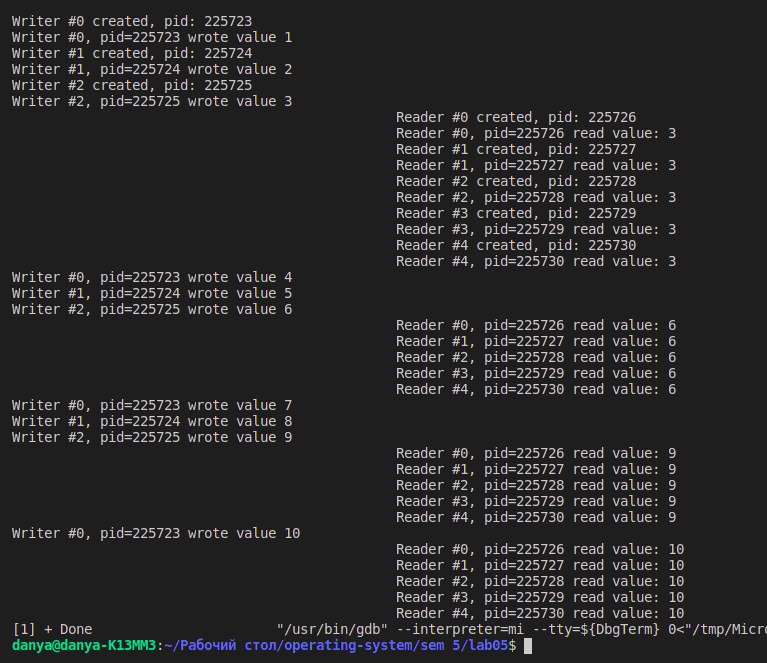
\includegraphics[scale=0.9]{task2.png}} 
	\caption{Пример работы программы №2}
	\label{ris:task2}
\end{figure}
\newpage
\begin{lstlisting}[label=three,caption =  Использование вызова exec(), style = CStyle]
#include <stdio.h>
#include <stdlib.h>
#include <unistd.h>

int main(){
	int child_1, child_2;
	child_1 = fork();
	if(child_1 == -1){
		perror("Coulnd't fork child #1");
		exit(1);
	}
	if (child_1 == 0){
		sleep(1);
		printf("\nChild #1 executes ps -al\n\n");
		if(execlp("ps", "ps", "-al", (char*)NULL) == -1){
			printf("Couldn't exec ps command\n");
			exit(1);
		}
		 
		 return 0;
	}
	if (child_1 > 0){
		child_2 = fork();
		if(child_2 == -1){
			perror("Coulnd't fork child #2");
			exit(1);
	        }
	        if (child_2 == 0){
	        	printf("\nChild #2 executes ls -l\n\n");
		 	if(execlp("ls", "ls", "-l", (char*)NULL) == -1){
				printf("Couldn't exec ps command\n");
				exit(1);
			}
		 return 0;
	        }else{
	       	printf("\nParent: pid=%d; group=%d; ppid=%d\n",
		  	 getpid(), getpgrp(), getppid());
		  	 
		  	pid_t child_pid;
		 	int status;
		 	
		 	//waiting for the second child to finish
		 	child_pid = wait(&status);
		 	if (WIFEXITED(status))
		 		printf("\nParent: child with pid = %d finished with code %d\n",
		 		 child_pid, WEXITSTATUS(status) );
		 	else if (WIFSTOPPED(status))
		 		printf("\nParent: child %d finished with code %d\n",
		 		 child_pid, WSTOPSIG(status) );
		 		 
		 	//waiting for the first child to finish	 
		 	child_pid = wait(&status);
		 	if (WIFEXITED(status))
		 		printf("\nParent: child with pid = %d finished with code %d\n",
		 		 child_pid, WEXITSTATUS(status) );
		 	else if (WIFSTOPPED(status))
		 		printf("\nParent: child %d finished with code %d\n",
		 		 child_pid, WSTOPSIG(status) );
		 
		 return 0;
	        }
	}
}
\end{lstlisting}
\begin{figure}[H]
	\centering{\includegraphics[scale=0.5]{task3.png}} 
	\caption{Пример работы программы №3}
	\label{ris:task3}
\end{figure}
\newpage
\begin{lstlisting}[label=four,caption = Передача сообщений с помощью программного канала, style = CStyle]
/*
exchanging messages with parent
*/
#include <stdio.h>
#include <stdlib.h>
#include <unistd.h>
#define MESSAGE_SIZE 32

int main(){
	int child_1, child_2;
	
	//initializing pipe
	int fd[2];
	if (pipe(fd) == -1){
		printf("Coundn't create a pipe\n");
		exit(1);
	}
	
	child_1 = fork();
	if(child_1 == -1){
		perror("Coulnd't fork child #1");
		exit(1);
	}
	if (child_1 == 0){
		
		 
		close(fd[0]);
		if (write(fd[1], "Hello from child #1, parent!\n",
		 MESSAGE_SIZE) > 0)
			printf("Child #1 sent a greeting to the parent\n");
		 return 0;
	}
	if (child_1 > 0){
		child_2 = fork();
		if(child_2 == -1){
			perror("Coulnd't fork child #2");
			exit(1);
	        }
	        if (child_2 == 0){
	        	sleep(1);
	        	close(fd[0]);
			if (write(fd[1], "Hello from child #2, parent!\n",
			 MESSAGE_SIZE) > 0)
				printf("Child #2 sent a greeting to the parent\n");
			 	return 0;
	        }else{
		  	
		  	char msg1[MESSAGE_SIZE], msg2[MESSAGE_SIZE];
			close(fd[1]);
			read(fd[0], msg1, MESSAGE_SIZE);
			read(fd[0], msg2, MESSAGE_SIZE);
			
			printf("Parent read a message from his children: \n%s\n%s",
			 msg1, msg2); 
			
			
			
		  	pid_t child_pid;
		 	int status;
		 	
		 	//waiting for the second child to finish
		 	child_pid = wait(&status);
		 	if (WIFEXITED(status))
		 		printf("\nParent: child with pid = %d finished with code %d\n",
		 		 child_pid, WEXITSTATUS(status) );
		 	else if (WIFSTOPPED(status))
		 		printf("\nParent: child %d finished with code %d\n",
		 		 child_pid, WSTOPSIG(status) );
		 		 
		 	//waiting for the first child to finish	 
		 	child_pid = wait(&status);
		 	if (WIFEXITED(status))
		 		printf("\nParent: child with pid = %d finished with code %d\n",
		 		 child_pid, WEXITSTATUS(status) );
		 	else if (WIFSTOPPED(status))
		 		printf("\nParent: child %d finished with code %d\n",
		 		 child_pid, WSTOPSIG(status) );
		 
		 return 0;
	        }
	}
}



\end{lstlisting}
\begin{figure}[H]
	\centering{\includegraphics[scale=0.7]{task4.png}} 
	\caption{Пример работы программы №4}
	\label{ris:task4}
\end{figure}
\newpage
\begin{lstlisting}[label=five,caption = Установка своего обработчика сигнала, style = CStyle]
/*
DIY sig handler
*/
#include <stdio.h>
#include <stdlib.h>
#include <unistd.h>
#include <signal.h>
#include <stdbool.h>
#include <string.h>

#define MESSAGE_SIZE 64
#define SLEEP_TIME 3

//flag is set to true if signal has been cought
bool flag = false;

void mySignalHandler(int snum){
	printf("\nHandlig signal snum = %d in prosses...\n", snum);
	printf("Done!\n");
	flag = true;
}

int main(){
	int child_1, child_2;
	signal(SIGINT, mySignalHandler);
	
	//initializing pipe
	int fd[2];
	if (pipe(fd) == -1){
		printf("Coundn't create a pipe\n");
		exit(1);
	}
	
	child_1 = fork();
	if(child_1 == -1){
		perror("Coulnd't fork child #1");
		exit(1);
	}
	if (child_1 == 0){
		close(fd[1]);
		sleep(SLEEP_TIME);
		if (flag){
			char msg[MESSAGE_SIZE];
			if (read(fd[0], msg, MESSAGE_SIZE) > 0){
				printf("Child #1 read from parent %s\n", msg);
			}
		}
		
		return 0;
	}
	if (child_1 > 0){
		child_2 = fork();
		if(child_2 == -1){
			perror("Coulnd't fork child #2");
			exit(1);
		}
		if (child_2 == 0){
			close(fd[1]);
			
			sleep(SLEEP_TIME);
			if (flag){
				char msg[MESSAGE_SIZE];
				if (read(fd[0], msg, MESSAGE_SIZE) > 0){
					printf("Child #2 read from parent %s\n", msg);
				}
			}
			
			return 0;
		}else{
			close(fd[0]);
			printf("Parent's waiting for Ctrl+C being pressed to send messages from children\n");
			sleep(SLEEP_TIME);
			
			if (flag){
				//writing in pipe if we cought the signal
				if (write(fd[1], "Hello, my child!\n", MESSAGE_SIZE) > 0)
				printf("Parent sent his first greeting\n");
				if (write(fd[1], "Hello again, my child!\n", MESSAGE_SIZE) > 0)
				printf("Parent sent his second greeting\n");
			}
		
			pid_t child_pid;
			int status;
			
			//waiting for the second child to finish
			child_pid = wait(&status);
			if (WIFEXITED(status))
			printf("Parent: child with pid = %d finished with code %d\n",
			child_pid, WEXITSTATUS(status) );
			else if (WIFSTOPPED(status))
			printf("Parent: child %d finished with code %d\n",
			child_pid, WSTOPSIG(status) );
			
			//waiting for the first child to finish	 
			child_pid = wait(&status);
			if (WIFEXITED(status))
			printf("Parent: child with pid = %d finished with code %d\n",
			child_pid, WEXITSTATUS(status) );
			else if (WIFSTOPPED(status))
			printf("Parent: child %d finished with code %d\n",
			child_pid, WSTOPSIG(status) );
			return 0;
		}
	}
}
\end{lstlisting}
\begin{figure}[H]
	\centering{\includegraphics[scale=1]{task5-1.png}} 
	\caption{Пример работы программы №5: был подан сигнал}
	\label{ris:task5-1}
\end{figure}
\begin{figure}[H]
	\centering{\includegraphics[scale=1]{task5-2.png}} 
	\caption{Пример работы программы №5: сигнал не был подан}
	\label{ris:task5-2}
\end{figure}
\newpage



\end{document}
